\chapter{Overview and reading guide}\label{ov:chapter}
\begingroup

This book is about one question: when does a quantum divergence between two channels, or an operational quantity that it bounds, depend continuously on the channels, and how large is the error when it does? Chapter~\ref{gate:chapter} has introduced the question through its physical motivation and stated the answers for characterized gates. Chapters~\ref{cont:chapter}--\ref{chn:chapter} develop the general theory, and Chapter~\ref{gate:proofschapter} contains the proofs of the results of Chapter~\ref{gate:chapter}. This chapter explains the organising idea of three classical ``shadows'' of a pair, the main results of each chapter and how the chapters depend on each other, and suggests reading orders. Chapter~\ref{nt:chapter} fixes the notation and records where the chapters differ in their conventions, and Chapter~\ref{op:chapter} collects the open problems.

\section{From noisy gates to the general questions}\label{ov:sec:problem}

The single-letter converses of Chapter~\ref{gate:chapter}, the geometric channel fidelity $\widehat F$, the geometric R\'enyi divergences $\widehat D_\alpha$ and the Belavkin--Staszewski relative entropy $D_{\mathrm{BS}}$, are each built from a Kubo--Ando mean of the Choi matrices of the two channels \cite{KatariyaWilde2021,FangFawzi2021}. That chapter showed how badly they can depend on the model of the channels. Their discontinuities are not limited to ideal gates: two pairs of replacement channels with the same sum can be arbitrarily close in the diamond norm and have geometric fidelities $0$ and $1$ (Corollary~\ref{cont:impossibility corollary}), just as an ideal unitary gate has geometric fidelity $1$ with itself and $0$ with every miscalibrated copy (Corollary~\ref{cont:cor:channels dichotomy}).

This raises several general questions, which organise the rest of the book.
\begin{enumerate}[(a)]
\item In which coordinates are these divergences continuous, and with which moduli? Where exactly are they discontinuous in the diamond norm?
\item Which divergences are continuous everywhere, and why?
\item Do the operational quantities, such as the Stein and Chernoff exponents of adaptive discrimination, share the discontinuities of their converses? When a converse jumps, does the task jump with it?
\item Near realistic noisy gates, where continuity holds, how large is the modulus, and how does it compare with the sensitivity of the task itself?
\end{enumerate}
Chapter~\ref{gate:chapter} answered~(d) and the physical side of~(c). The answers to~(a)--(c) depend on the family of divergences, and the main structural message is that each family is a functional of a different classical object attached to the pair.

\section{Three shadows of a pair}\label{ov:sec:shadows}

For a pair of positive operators, or of completely positive maps, there are several ways to extract a classical pair of measures, and each of the standard families of quantum divergences is a classical divergence of one of them. We call these classical objects the \emph{shadows} of the pair. Three of them carry most of this book.

\emph{(I) The reverse test.} For states $\rho,\sigma$ with $\omega=\rho+\sigma$, the operator $T=\omega^{-1/2}\rho\,\omega^{-1/2}$ (on the support of $\omega$) is a positive contraction, and its spectral measure in the state $\omega$ gives a classical pair. Its classical divergences are the maximal $f$-divergences of Matsumoto \cite{Matsumoto2018newf} and the Kubo--Ando means; in particular $\widehat F$, $\widehat D_\alpha$ and $D_{\mathrm{BS}}$ belong to this family. For completely positive maps the role of $T$ is played by the Arveson--Radon--Nikodym (ARN) derivative of $\Phi$ with respect to $\Omega=\Phi+\Psi$: if $\Omega$ has linearly independent Kraus operators $V_1,\dots,V_r$, then $\Phi(X)=\sum_{k,l}T_{kl}V_kXV_l^*$ for a unique $0\le T\le\mathbf 1$ (Theorem~\ref{cont:thm:arveson}). Its transpose is the effect, on the environment of a Stinespring dilation of $\Omega$, that selects the branch $\Phi$ (Theorem~\ref{cont:effect theorem}). Every Kubo--Ando mean of the Choi matrices is $W g_\sigma(T)W^*$ for a scalar function $g_\sigma$ and the matrix $W$ of Kraus vectors (Theorem~\ref{cont:fundamental principle}). This is the shadow of Chapters~\ref{cont:chapter} and~\ref{chn:chapter}.

\emph{(II) The testing region.} The hockey-stick profile $e(\gamma)=\Tr(\rho-\gamma\sigma)_+$, $\gamma\ge0$, encodes all the binary tests between $\rho$ and $\sigma$. Its second derivative $\mu=e''$ is a measure on $(0,\infty)$, completed by boundary atoms at $0$ and $\infty$. The hypothesis-testing quantities, the Hirche--Tomamichel $f$-divergences \cite{HircheTomamichel2024} and, by Frenkel's formula \cite{Frenkel2023}, the Umegaki relative entropy are functionals of this shadow. It is the shadow of Chapters~\ref{shA:chapter} and~\ref{shB:chapter}.

\emph{(III) The modular shadow.} The Nussbaum--Szko{\l}a pair of the relative modular operator \cite{NussbaumSzkola2009} gives the Petz $f$-divergences. Through the modular derivative $\widetilde T=\Delta(\mathbf 1+\Delta)^{-1}$ it can be treated with the same tools as the reverse test (Section~\ref{shA:sec:petz}).

Two further families appear as limits or suprema of these: the measured divergences, a supremum over many classical pairs, and the sandwiched and regularised divergences, which appear only after tensor powers. Section~\ref{shA:sec:summary} contains a table that places all five families side by side.

The three shadows are ordered. The testing-region shadow is a garbling of the reverse test (Theorem~\ref{shA:thm:Tlift}), and the modular shadow has the boundary masses of the testing region, not those of the reverse test (Theorem~\ref{shA:thm:modular}). This ordering explains the difference in continuity. The reverse test can be destroyed by an $O(\sqrt t)$ perturbation that couples the kernel of the sum to its range, so the obstruction to continuity for family~(I) is the invertibility of the sum $J(\Phi+\Psi)$. The testing region does not see that mechanism, and the only obstruction left for family~(II) is a leak of support, which is controlled by the invertibility of the second argument.

\section{Results by chapter}\label{ov:sec:results}

The results of Chapter~\ref{gate:chapter} are listed in its introduction and are not repeated here. The other chapters contain the following main results.

\subsection*{Chapter~\ref{cont:chapter}: continuity of Kubo--Ando channel divergences}

Chapter~\ref{cont:chapter} develops family~(I) for completely positive maps. Since every quantity of the family is a scalar function of the ARN derivative, read through the Kraus operators of the sum, it is continuous in $T$ with a dimension-free constant. For the fidelity,
\[
\big|\widehat F(\Phi_1,\Psi_1)-\widehat F(\Phi_2,\Psi_2)\big|\le\|\Omega^*(\mathbf 1_{\mathcal Y})\|_\infty\,\|T_1-T_2\|_\infty^{1/2}
\]
for two pairs with the same sum $\Omega$, and the constant and the exponent are sharp (Theorem~\ref{cont:main theorem}). Analogous bounds hold for all means, for $\widehat Q_\alpha$ with $\alpha\in(0,1)$ and for bounded maximal $f$-divergences (Theorems~\ref{cont:Modulus of continuity results}, \ref{cont:thm:renyi continuity} and~\ref{cont:thm:maxf}), and, under a bound on $D_{\max}$ within each pair, for $D_{\mathrm{BS}}$ and $\widehat Q_\alpha$ with $\alpha\in(1,2]$ (Theorem~\ref{cont:thm:unbounded}). Every maximal $f$-divergence of an operator convex $f$ has a closed form as the largest eigenvalue of a partial trace and is continuous in $T$ with values in $(-\infty,+\infty]$ (Theorems~\ref{cont:thm:all f} and~\ref{cont:thm:extended continuity}). Section~\ref{cont:sec:loewner} gives explicit moduli for every mean and every operator convex $f$.

The passage to the diamond norm goes through the quantity $\nu(\Omega)$, the smallest operator norm of a unit combination of the Kraus operators of the sum, which bounds the derivative distance by the diamond distance (Theorem~\ref{cont:thm:two sided}, Corollary~\ref{cont:cor:cb continuity}). Pairs with different sums are compared through the Thompson metric (Theorem~\ref{cont:thm:four maps}, Corollary~\ref{cont:cor:universal}), and support changes through the Lebesgue decomposition of the sums (Theorem~\ref{cont:thm:different supports}). The main structural result is a dichotomy (Theorem~\ref{cont:thm:dichotomy}): on pairs of completely positive maps, $\widehat F$ is continuous at $(\Phi,\Psi)$ if and only if $J(\Phi+\Psi)$ is invertible or $\widehat F(\Phi,\Psi)=0$, with analogues for the other quantities. Within channels the dichotomy holds at diagonal pairs $(\Phi,\Phi)$, where output rotations already produce the jump (Theorem~\ref{cont:thm:channel orbit}, Corollary~\ref{cont:cor:diagonal channels}), and zero-temperature amplitude damping jumps from $1$ to $0$ within its own family (Example~\ref{cont:ex:amplitude damping}). Quantitatively, if the Choi matrices are bounded below by $\lambda>0$, the fidelity is Lipschitz in the diamond norm with a relative constant of the sharp order $\lambda^{-1}$ (Theorem~\ref{cont:thm:choi floor}, Example~\ref{cont:ex:choi floor sharp}), and at mutually singular pairs it tends to zero at the sharp rate $d^{1/2}/\sin\theta$ (Theorem~\ref{cont:thm:singular rate}).

\subsection*{Chapter~\ref{shA:chapter}: testing regions, modular lifts and continuity}

Chapter~\ref{shA:chapter} carries the programme of Chapter~\ref{cont:chapter} through families~(II)--(V). The testing-region shadow has atoms exactly at the relative spectrum, dominated by those of the reverse test, and an absolutely continuous part whose density is the coupling of $\sigma$ across the Helstrom test (Theorems~\ref{shA:thm:structure} and~\ref{shA:thm:Tlift}). One consequence is an explicit nonnegative integral formula for $D_{\mathrm{BS}}-D$, and another is that the measured, testing-region and maximal divergences of a strictly convex function coincide only for commuting pairs (Corollary~\ref{shA:cor:rigidity}). Every testing-region $f$-divergence with finite boundary values is uniformly continuous with a dimension-free modulus, so these divergences have no dichotomy (Theorem~\ref{shA:thm:bounded}, Corollary~\ref{shA:cor:nodichotomy}), and the Umegaki relative entropy is continuous at $(\rho,\sigma)$ exactly when $\sigma$ is invertible or $D(\rho\|\sigma)=\infty$ (Theorem~\ref{shA:thm:unbounded}). Bounded Petz divergences are continuous everywhere, with a dimension-free H\"older modulus (Theorem~\ref{shA:thm:petzcont}).

For channels the chapter replaces the trace norm by the Thompson metric of the Choi matrices and the relative entropy by a conditional entropy. Every $n$-use adaptive quantity of a suitable divergence is $n\,d_{\mathrm T}$-Lipschitz in the second channel (Theorem~\ref{shA:thm:thompson}), and the first argument is controlled uniformly over references (Theorem~\ref{shA:thm:firstarg}). Together these give an explicit modulus for the adaptive Stein exponent $\zeta$, and the analogue of the dichotomy: $\zeta$ is continuous at $(\Phi,\Psi)$ if and only if $J(\Psi)$ is invertible or $\zeta(\Phi,\Psi)=\infty$ (Corollary~\ref{shA:cor:stein}). The chapter also treats the strong-converse exponent and the regularised sandwiched and Petz divergences (Theorems~\ref{shA:thm:sandfirst} and~\ref{shA:thm:petzfirst}, Corollary~\ref{shA:cor:sand}), and gives an exact one-shot dual formula for testing-region channel divergences together with their regularised values (Theorems~\ref{shA:thm:oneshot} and~\ref{shA:thm:htreg}).

\subsection*{Chapter~\ref{shB:chapter}: super-multiplicativity of hockey-stick R\'enyi quasi-entropies}

The reverse test and the modular shadow factorise under tensor products, but the testing region does not. Chapter~\ref{shB:chapter} studies what replaces multiplicativity for the testing-region R\'enyi quasi-entropies $Q^{\mathrm{HT}}_\alpha$, the Mellin moments of the hockey-stick profile. Conjecture~\ref{shB:conj:super} asserts that they are super-multiplicative, so that $D^{\mathrm{HT}}_\alpha$ is superadditive for $\alpha>1$ and subadditive for $\alpha<1$. The chapter proves the conjecture at $\alpha=2$ (Theorem~\ref{shB:thm:super2}), at every integer order for pure states and at $\alpha=3$ for sign-free pairs (Theorem~\ref{shB:thm:simplex}), at every integer order against pure partners (Theorem~\ref{shB:thm:purepartner}), at $\alpha=3$ whenever one reference state has at most two distinct eigenvalues (Corollary~\ref{shB:cor:twolevel}), for one measured factor (Theorem~\ref{shB:thm:supermeas}), to first order as $\alpha\to\infty$ (Theorem~\ref{shB:thm:superinf}) and for tensor powers with enough copies (Proposition~\ref{shB:prop:manycopies}). Structurally, the conjecture is the family of moment inequalities of a convex-order domination between two Frenkel measures (Theorem~\ref{shB:thm:frenkel}). One-way LOCC tests never beat the classical product of the shadows (Proposition~\ref{shB:prop:oneway}), so a proof must use entangled tests. The chapter also gives an elementary proof of $D^{\mathrm{HT}}_\alpha\le\widetilde D_\alpha$ for $\alpha\ge2$ (Theorem~\ref{shB:thm:bht2}). Unlike the other chapters, it is a chapter of matrix analysis: continuity plays no role, and quantum channels appear only as garblings between a pair and its shadow (Section~\ref{shB:sec:restricted}).

\subsection*{Chapter~\ref{chn:chapter}: adaptive discrimination as a controlled random walk}

Chapter~\ref{chn:chapter} turns the ARN derivative into a converse for adaptive discrimination. Diagonalising $T=\sum_\ell\tau_\ell P_\ell$ writes the pair as $\Phi=\sum_\ell\tau_\ell\Omega_\ell$ and $\Psi=\sum_\ell(1-\tau_\ell)\Omega_\ell$ with common completely positive level maps $\Omega_\ell$ (Lemma~\ref{chn:lem:levels}). Each use of the unknown channel therefore selects a level and then acts in a way that does not depend on the hypothesis, and every adaptive protocol is a post-processing of a controlled random walk whose step values are fixed (Proposition~\ref{chn:prop:walk}). The result is the geometric Chernoff converse: every adaptive strategy errs with probability at least $\frac14\exp(-n\widehat C-\sqrt{2\ln4}\,\Lambda\sqrt n)$, where $\widehat C=-\ln\min_s\lambda_{\min}(B_s)$ is computable from one eigendecomposition (Theorem~\ref{chn:thm:main}). No other common decomposition gives a better bound of this kind (Proposition~\ref{chn:prop:canon}); $\widehat C$ lies between one half of the fidelity converse and the fidelity converse and is not comparable with the barycentric converse (Corollary~\ref{chn:cor:compare}, Proposition~\ref{chn:prop:bary}). If the levels are orthogonal at an optimal input, product strategies attain $\widehat C$ (Theorems~\ref{chn:thm:tight} and~\ref{chn:thm:exact}).

The continuity section applies Chapter~\ref{cont:chapter} to the converse itself. Under perturbations that are small relative to the pair, $e^{-\widehat C}$ is Lipschitz (Theorem~\ref{chn:thm:robust}), which gives a converse valid for a whole neighbourhood of a model pair (Corollary~\ref{chn:cor:uncertain}); under general perturbations it is only lower semicontinuous, and continuous where $J(\Phi+\Psi)$ is invertible (Theorem~\ref{chn:thm:semicont}). Near replacement channels with rank-deficient outputs, the fidelity, barycentric and geometric Chernoff converses are all infinite while the adaptive exponent tends to zero (Theorem~\ref{chn:thm:fragile}). The same happens for amplitude-damping channels with nearby damping rates, where a pure-program simulation gives a finite converse of the right order (Theorem~\ref{chn:thm:pureprog}, Corollary~\ref{chn:cor:adfragile}).

\subsection*{Chapter~\ref{gate:proofschapter}: noisy gates, proofs and further results}

Chapter~\ref{gate:proofschapter} proves the results that Chapter~\ref{gate:chapter} states for characterized gates: the classification of discontinuities into genuine, spurious and absent by the supports of Choi matrices, the Choi-floor law $\ln[1/(1-r)]$ with $r=\epsilon/(2\tilde\lambda)$ and its sharpness (Section~\ref{gate:sec:floor}), the equality of converses and exponents at the worst case (Section~\ref{gate:sec:m1first}), and the comparison of the converses with the adaptive Stein and Chernoff exponents under a coherent miscalibration, locally and at finite miscalibration (Sections~\ref{gate:sec:local}, \ref{gate:sec:m1chernoff} and~\ref{gate:sec:finite}). It also contains closed forms of the divergences and of the asymptotic adaptive Fisher information for all Pauli channels and Pauli-string miscalibrations (Sections~\ref{gate:sec:pauli}, \ref{gate:sec:window} and~\ref{gate:sec:biased}), the analysis of amplitude damping and of the program-simulation converse (Section~\ref{gate:sec:ad}), the certification bounds (Section~\ref{gate:sec:cert-proofs}) and the numerical methods (Section~\ref{gate:sec:methods}). Section~\ref{gate:smp:sec} points to the results of Chapters~\ref{cont:chapter}, \ref{shA:chapter} and~\ref{chn:chapter} that these proofs use and proves the refinements of them that are needed.

\section{How the chapters depend on each other}\label{ov:sec:dependencies}

Figure~\ref{ov:fig:dependencies} shows the logical dependencies. Chapter~\ref{gate:chapter} comes first because it frames the theory, but it states its results with forward references: they are proved in Chapter~\ref{gate:proofschapter}, with the help of Chapters~\ref{cont:chapter}, \ref{shA:chapter} and~\ref{chn:chapter}. Chapter~\ref{cont:chapter} is the foundation: it introduces the ARN derivative, the Thompson metric between sums, the relative distance of two pairs and the dichotomy. Chapter~\ref{shA:chapter} uses the reverse test of Chapter~\ref{cont:chapter} as the reference point for the testing region and the modular shadow, and compares its continuity results with the dichotomy. Chapter~\ref{shB:chapter} uses the definitions and the tensor-product sandwiches of Chapter~\ref{shA:chapter}. Chapter~\ref{chn:chapter} uses the derivative, the level decomposition it induces, and the continuity estimates for pairs with different sums from Chapter~\ref{cont:chapter}. Chapter~\ref{gate:proofschapter} draws on all three of Chapters~\ref{cont:chapter}, \ref{shA:chapter} and~\ref{chn:chapter}: the Choi-floor estimates and the dichotomy, the continuity of the Stein exponent, and the geometric Chernoff converse with its fragility. Together, Chapters~\ref{gate:chapter} and~\ref{gate:proofschapter} are largely self-contained. Chapters~\ref{shB:chapter} and~\ref{chn:chapter} are linked only through an open problem, which asks whether the adaptive Chernoff exponent is a regularised testing-region quantity (Problem~\ref{op:prob:chernoff testing}).

\begin{figure}[htbp]
\centering
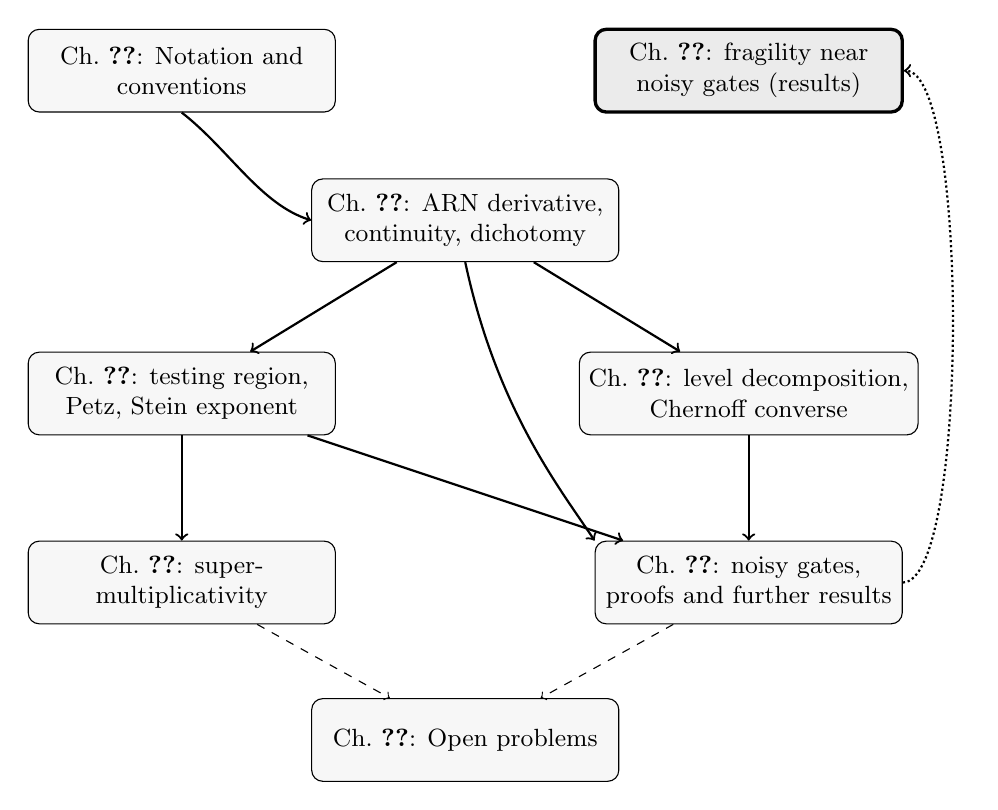
\begin{tikzpicture}[
  every node/.style={font=\small},
  box/.style={draw, rounded corners, align=center, minimum width=3.9cm, minimum height=1.05cm, fill=black!3},
  entry/.style={box, very thick, fill=black!8},
  dep/.style={->, thick},
  proof/.style={->, thick, densely dotted},
  weak/.style={->, dashed}
]
\node[entry] (c1) at (3.6,1.9) {Ch.~\ref{gate:chapter}: fragility near\\ noisy gates (results)};
\node[box] (c3) at (-3.6,1.9) {Ch.~\ref{nt:chapter}: Notation and\\ conventions};
\node[box] (c4) at (0,0) {Ch.~\ref{cont:chapter}: ARN derivative,\\ continuity, dichotomy};
\node[box] (c5) at (-3.6,-2.2) {Ch.~\ref{shA:chapter}: testing region,\\ Petz, Stein exponent};
\node[box] (c7) at (3.6,-2.2) {Ch.~\ref{chn:chapter}: level decomposition,\\ Chernoff converse};
\node[box] (c6) at (-3.6,-4.6) {Ch.~\ref{shB:chapter}: super-\\ multiplicativity};
\node[box] (c8) at (3.6,-4.6) {Ch.~\ref{gate:proofschapter}: noisy gates,\\ proofs and further results};
\node[box] (c9) at (0,-6.6) {Ch.~\ref{op:chapter}: Open problems};
\draw[dep] (c3.south) .. controls (-3.0,0.9) and (-2.6,0.2) .. (c4.west);
\draw[dep] (c4) -- (c5);
\draw[dep] (c4) -- (c7);
\draw[dep] (c5) -- (c6);
\draw[dep] (c7) -- (c8);
\draw[dep] (c5) -- (c8);
\draw[dep] (c4.south) .. controls (0.4,-2.4) and (1.2,-3.4) .. (c8.north west);
\draw[proof] (c8.east) .. controls (6.4,-4.6) and (6.4,1.9) .. (c1.east);
\draw[weak] (c6) -- (c9);
\draw[weak] (c8) -- (c9);
\end{tikzpicture}
\caption{Dependencies between the chapters. A solid arrow means that the chapter at its head uses definitions or results of the chapter at its tail. The book opens with Chapter~\ref{gate:chapter} (thick frame), which states results proved in Chapter~\ref{gate:proofschapter} (dotted arrow). Dashed arrows indicate that the open problems draw on every chapter.}
\label{ov:fig:dependencies}
\end{figure}

There are also some overlaps that we have kept. Chapter~\ref{shB:chapter} recalls the definitions of the testing region in a compact form, and Chapter~\ref{gate:chapter} restates the results it needs from Chapters~\ref{cont:chapter}, \ref{shA:chapter} and~\ref{chn:chapter} so that it can be read on its own, before them; in both cases the restatements point to the original results.

\section{A reading guide}\label{ov:sec:reading}

The chapters after this one can be read in several orders.

\emph{Mathematicians} interested in operator theory and matrix analysis can read Chapter~\ref{cont:chapter} in order: Sections~\ref{cont:sec:prelim}--\ref{cont:sec:norms} contain the ARN derivative, the Kubo--Ando background and the basic continuity estimate, and Section~\ref{cont:sec:dichotomy} the dichotomy. Chapter~\ref{shA:chapter} follows naturally, with Sections~\ref{shA:sec:shadows}--\ref{shA:sec:petz} on states. Chapter~\ref{shB:chapter} can be read directly after Section~\ref{shA:sec:shadows}; it is the most self-contained chapter and needs no channels.

\emph{Information theorists} interested in converse bounds for discrimination can continue with Chapter~\ref{chn:chapter}, which needs only the ARN theorem (Theorem~\ref{cont:thm:arveson}) and, in its continuity section, the estimates of Section~\ref{cont:sec:different sums}. Section~\ref{shA:sec:channels} contains the corresponding results for the Stein exponent and the strong-converse exponent.

\emph{Physicists} interested in noisy gates and their characterization will find the results in Chapter~\ref{gate:chapter}, which states them operationally and defines every symbol it uses, and their proofs in Chapter~\ref{gate:proofschapter}. The remarks headed ``Physical interpretation'' in Chapter~\ref{cont:chapter} explain the derivative, the quantity $\nu(\Omega)$ and the dichotomy in terms of instruments and environments, and Section~\ref{cont:sec:four maps} contains the Choi-floor estimates in their original form.

Readers who move between chapters should consult Chapter~\ref{nt:chapter}. Each chapter keeps its own notation, and the conventions differ in a few places, most importantly in the ordering of tensor factors in the Choi matrix, in whether the fidelity of states is squared, and in the notation for the (natural) logarithm (Table~\ref{nt:tab:differences}).

\section{About this book}\label{ov:sec:edition}

Chapter~\ref{cont:chapter} is a revised and extended version of \cite{Jones2026}. Theorems are numbered by chapter and section, and every cross-reference between chapters is internal.

\subsection*{Numerical verification}
The results of this book have been checked numerically. Every result of Chapter~\ref{cont:chapter} went through an independent, computer-assisted audit: its proofs were re-derived, and every formula and constant was tested numerically, in $50$--$110$-digit arithmetic near singular points and with diamond norms and Schur-multiplier norms computed exactly by semidefinite programming. No statement was found to be false and no proof was found to have a gap; the minor corrections the audit produced (missing hypotheses, edge cases and one display) are incorporated in Chapter~\ref{cont:chapter}. Every numerical value, table and figure in Chapters~\ref{gate:chapter} and~\ref{gate:proofschapter} and in Section~\ref{chn:sec:ad}, and the hockey-stick estimate of Chapter~\ref{shA:chapter}, is reproduced by a script, and the proved statements of those chapters were cross-checked numerically. The code, the data, the audit scripts and the audit reports are in the \texttt{code/} directory of the repository that accompanies this book, \url{https://github.com/mjones1298/Continuity-of-divergences-python-}: \texttt{code/README.md} maps each claim to the script that produces it, and \texttt{code/audit\_ch04/} contains the audit of Chapter~\ref{cont:chapter}. The numerical checks reported in Sections~\ref{shA:sec:numerics}, \ref{shB:sec:numerics} and~\ref{chn:sec:num} were computed with the author's own code, which is not included.

\endgroup
